\chapter{Extra Information}

\section{Figures}
\begin{figure}[h]
	\makebox[\textwidth][c]{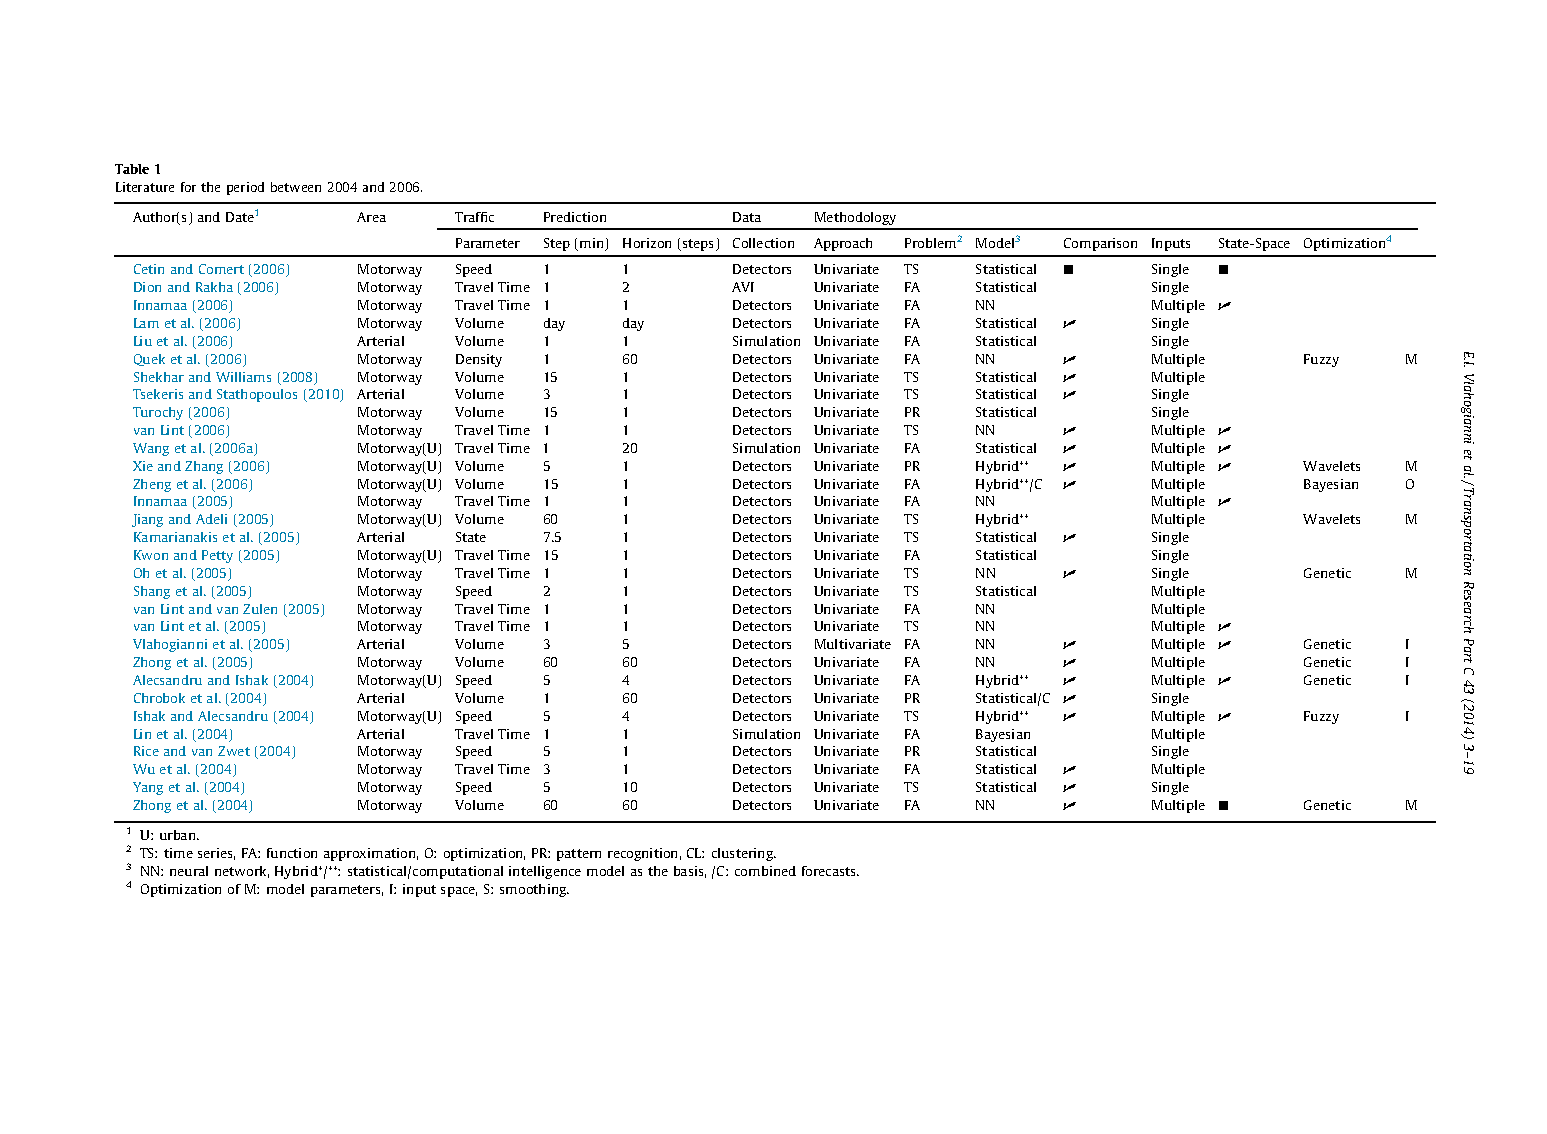
\includegraphics[page=1, width=1.8\textwidth]{Figures/shortTermForecastResearchTable.pdf}}
	\caption{Short-term traffic forecasting research taken from \cite{Vlahogianni20143}}
	\label{fig:Vlahogianni201431}
\end{figure}

\begin{figure}[ht]
	\makebox[\textwidth][c]{\includegraphics[page=2, width=1.8\textwidth]{Figures/shortTermForecastResearchTable.pdf}}
	\caption{Short-term traffic forecasting research taken from \cite{Vlahogianni20143}}
	\label{fig:Vlahogianni201432}
\end{figure}

\begin{figure}[ht]
	\makebox[\textwidth][c]{\includegraphics[page=3, width=1.8\textwidth]{Figures/shortTermForecastResearchTable.pdf}}
	\caption{Short-term traffic forecasting research taken from \cite{Vlahogianni20143}}
	\label{fig:Vlahogianni201433}
\end{figure}

\begin{figure}[ht]
	\makebox[\textwidth][c]{\includegraphics[page=4, width=1.8\textwidth]{Figures/shortTermForecastResearchTable.pdf}}
	\caption{Short-term traffic forecasting research taken from \cite{Vlahogianni20143}}
\label{fig:Vlahogianni201434}
\end{figure}

\FloatBarrier
\section{Design Diagrams}
%USE CASE DIAGRAM
\begin{figure}
	\makebox[\textwidth][c]{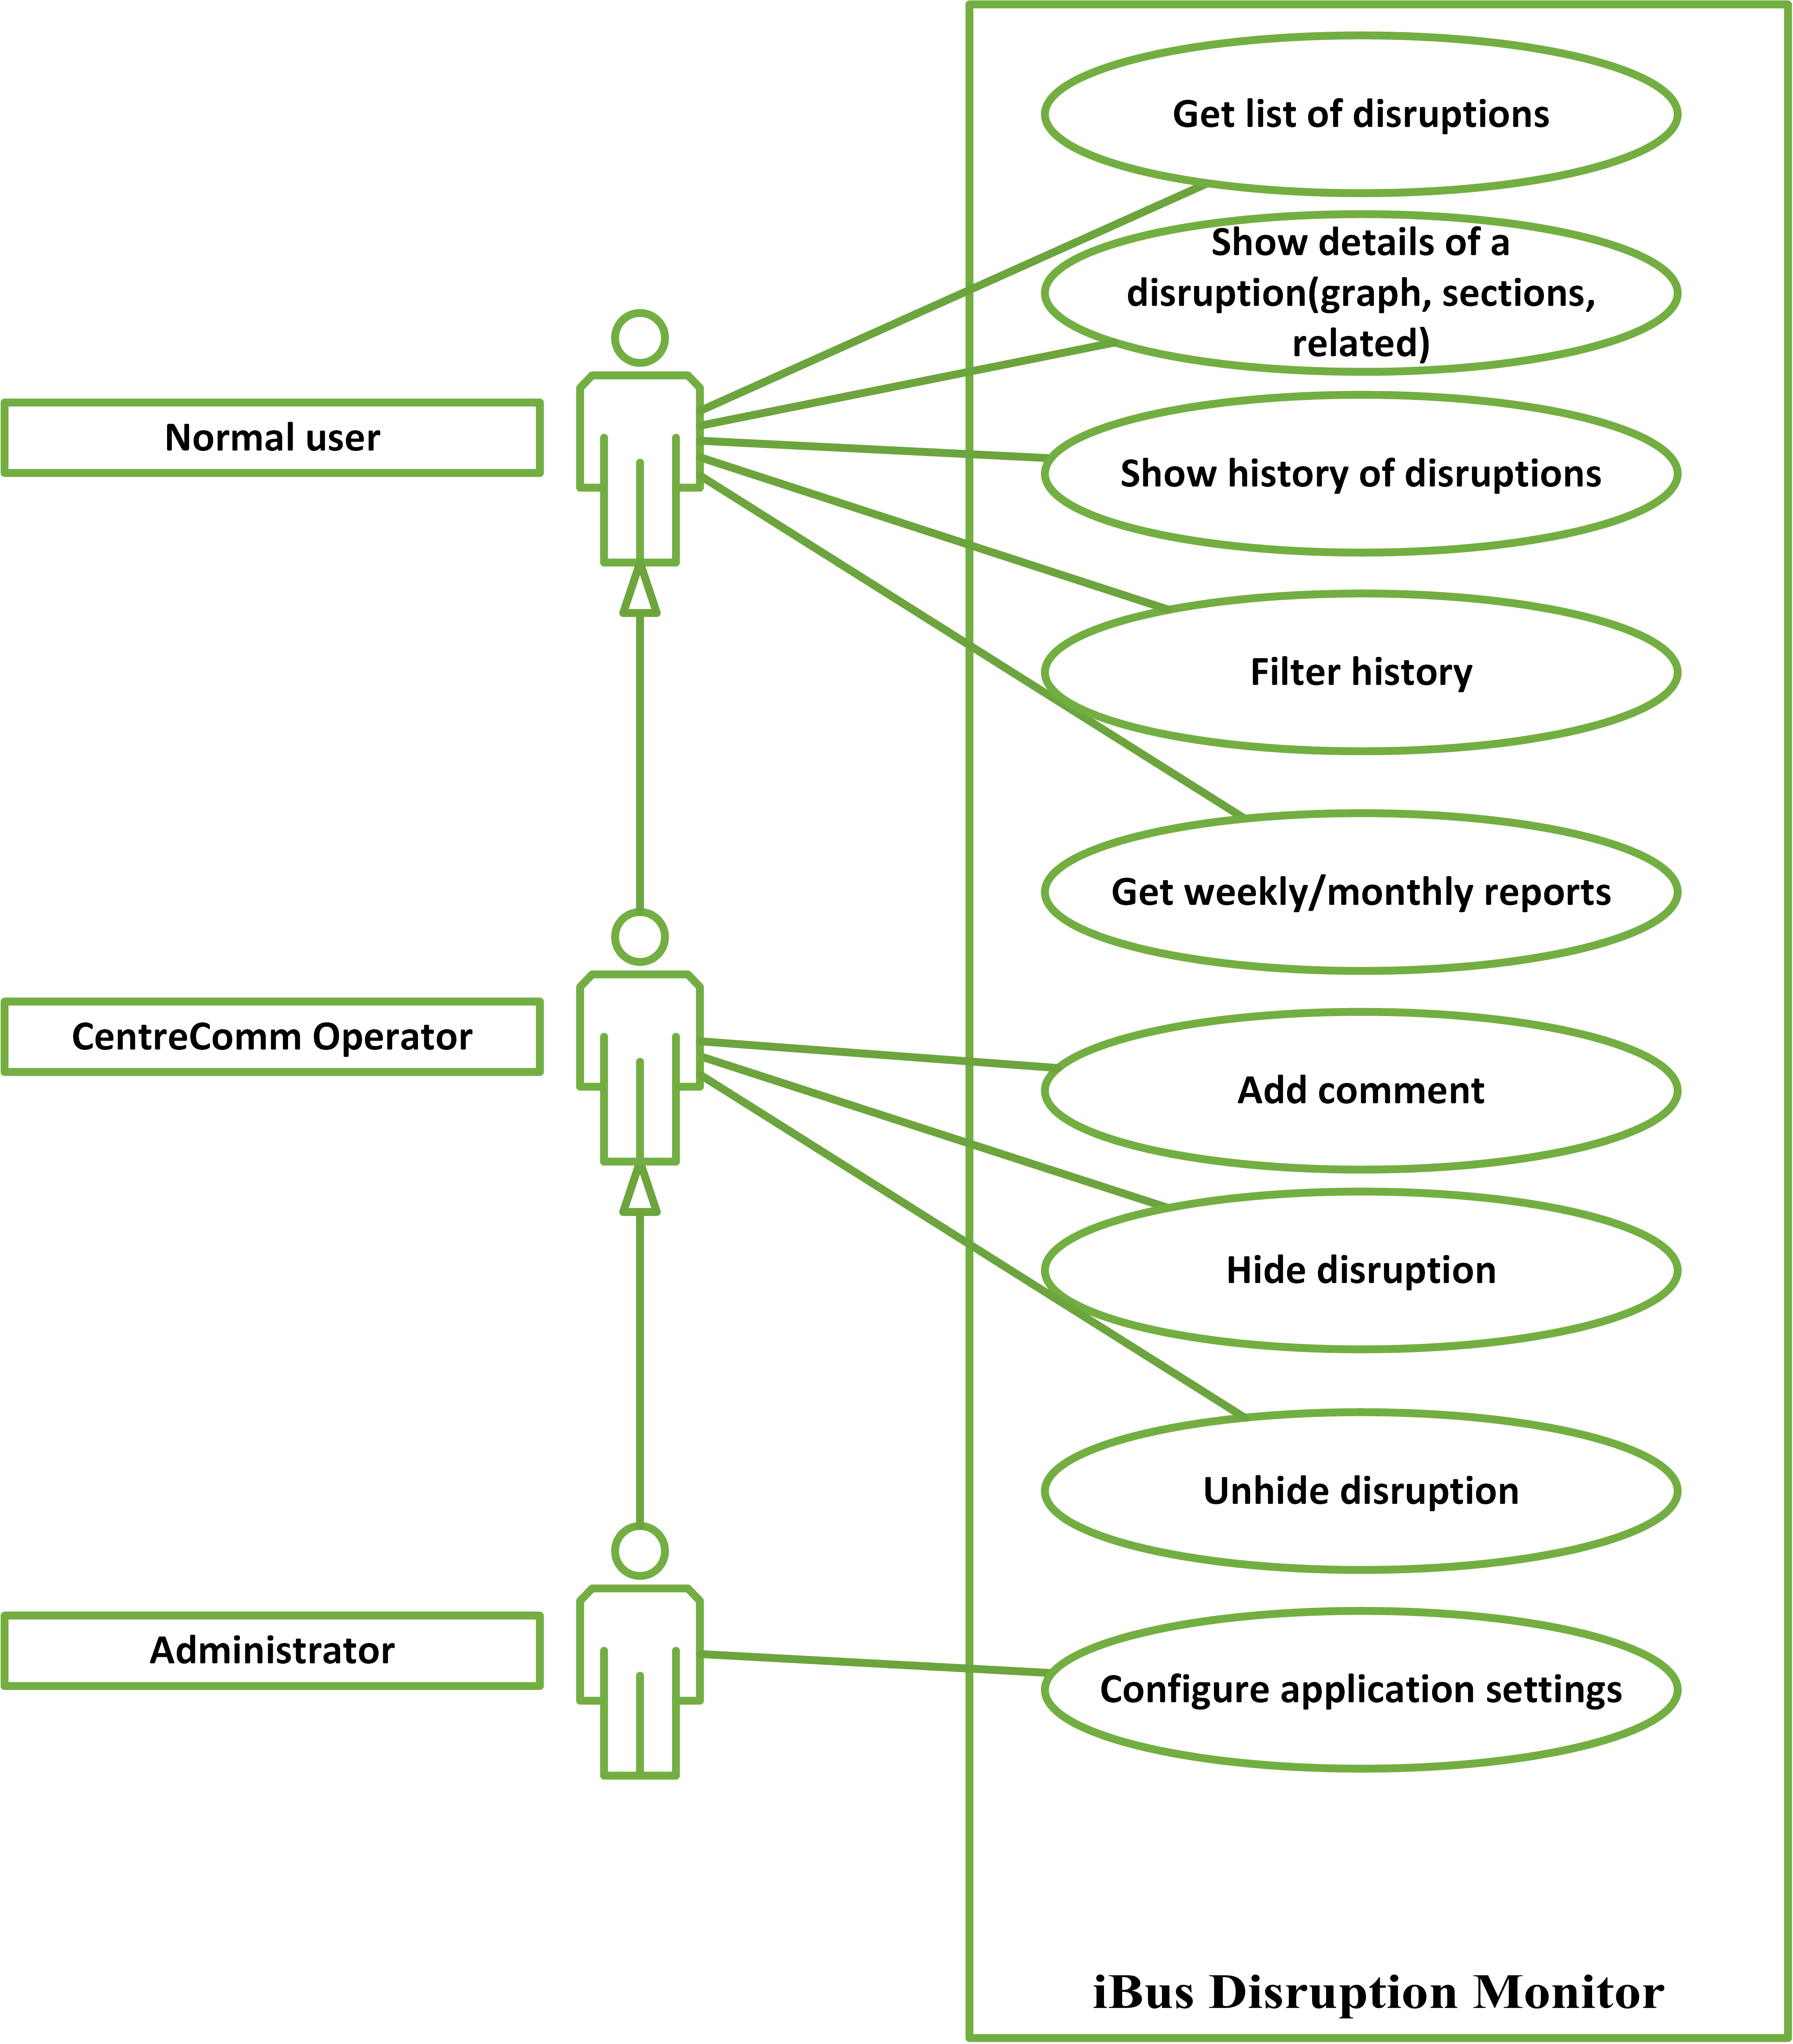
\includegraphics[width=1.2\textwidth]{Figures/UseCases.png}}
	\caption{Use Case Diagram}
\label{fig:useCase}
\end{figure}
%ARCHITECTURE DIAGRAM
\begin{figure}
	\makebox[\textwidth][c]{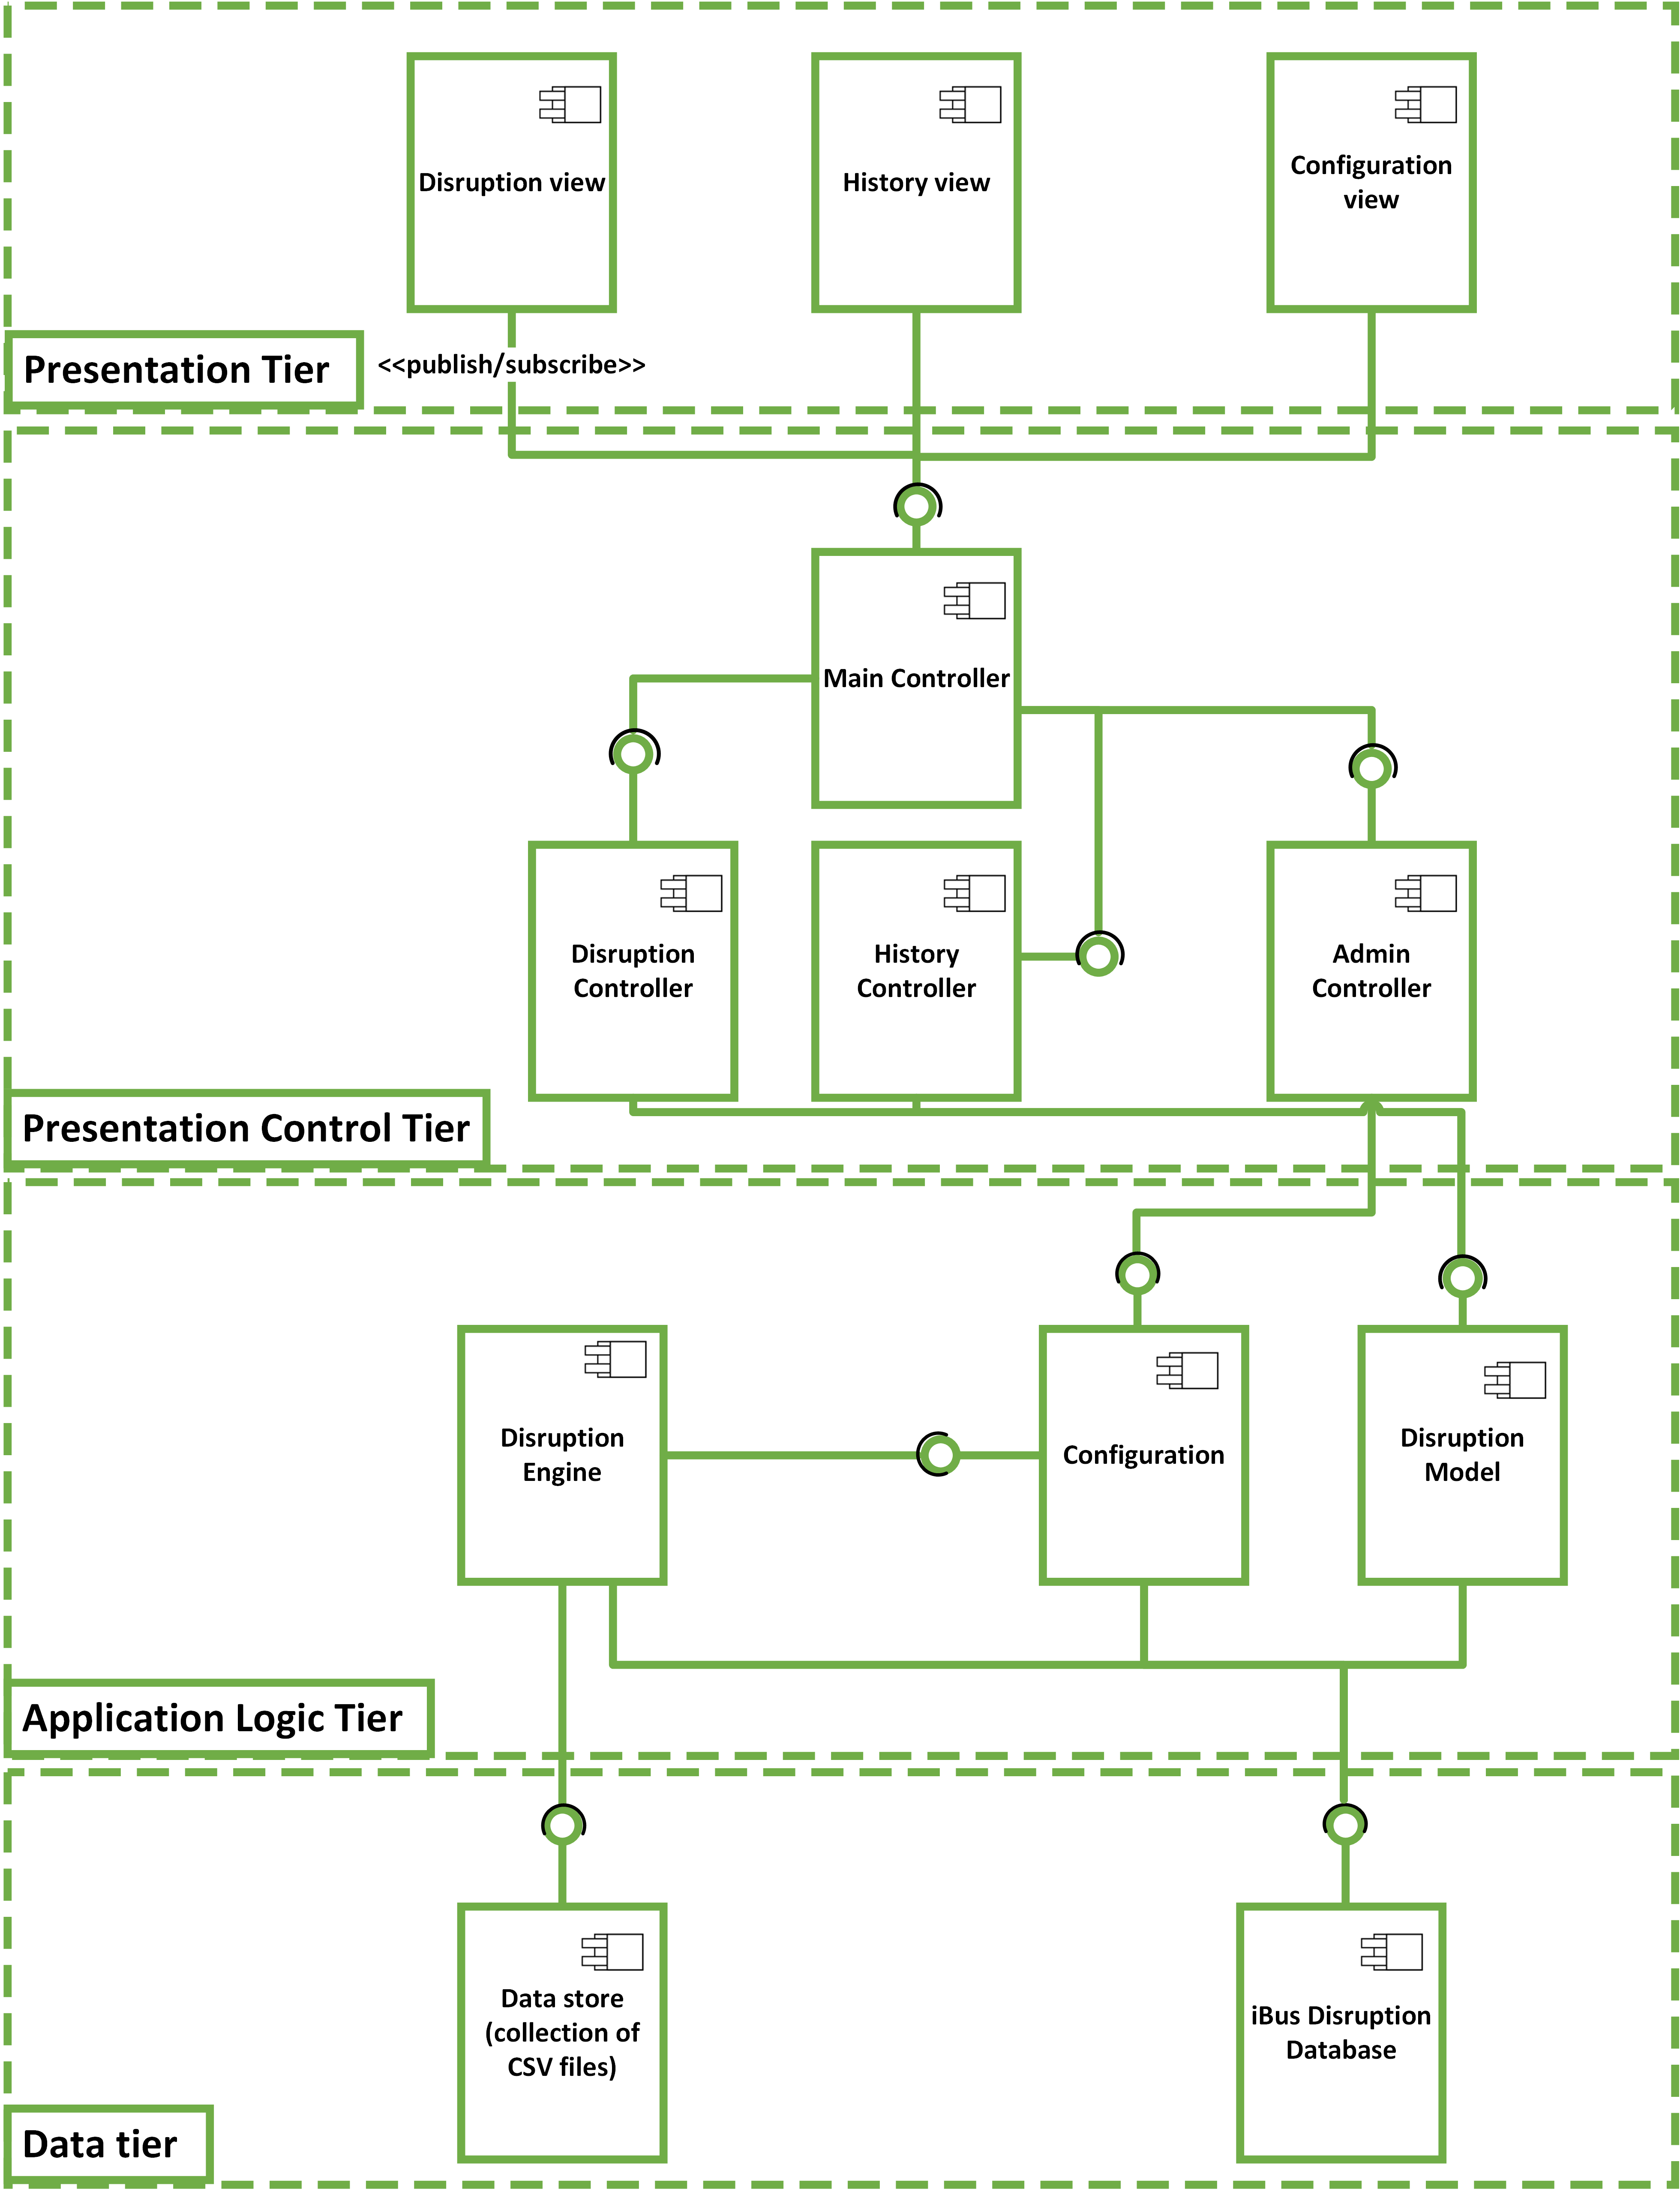
\includegraphics[width=1.2\textwidth]{Figures/Architecture.png}}
	\caption{System Architecture Diagram}
\label{fig:systemArchitecture}
\end{figure}
%CLASS DIAGRAM
\begin{figure}
	\makebox[\textwidth][c]{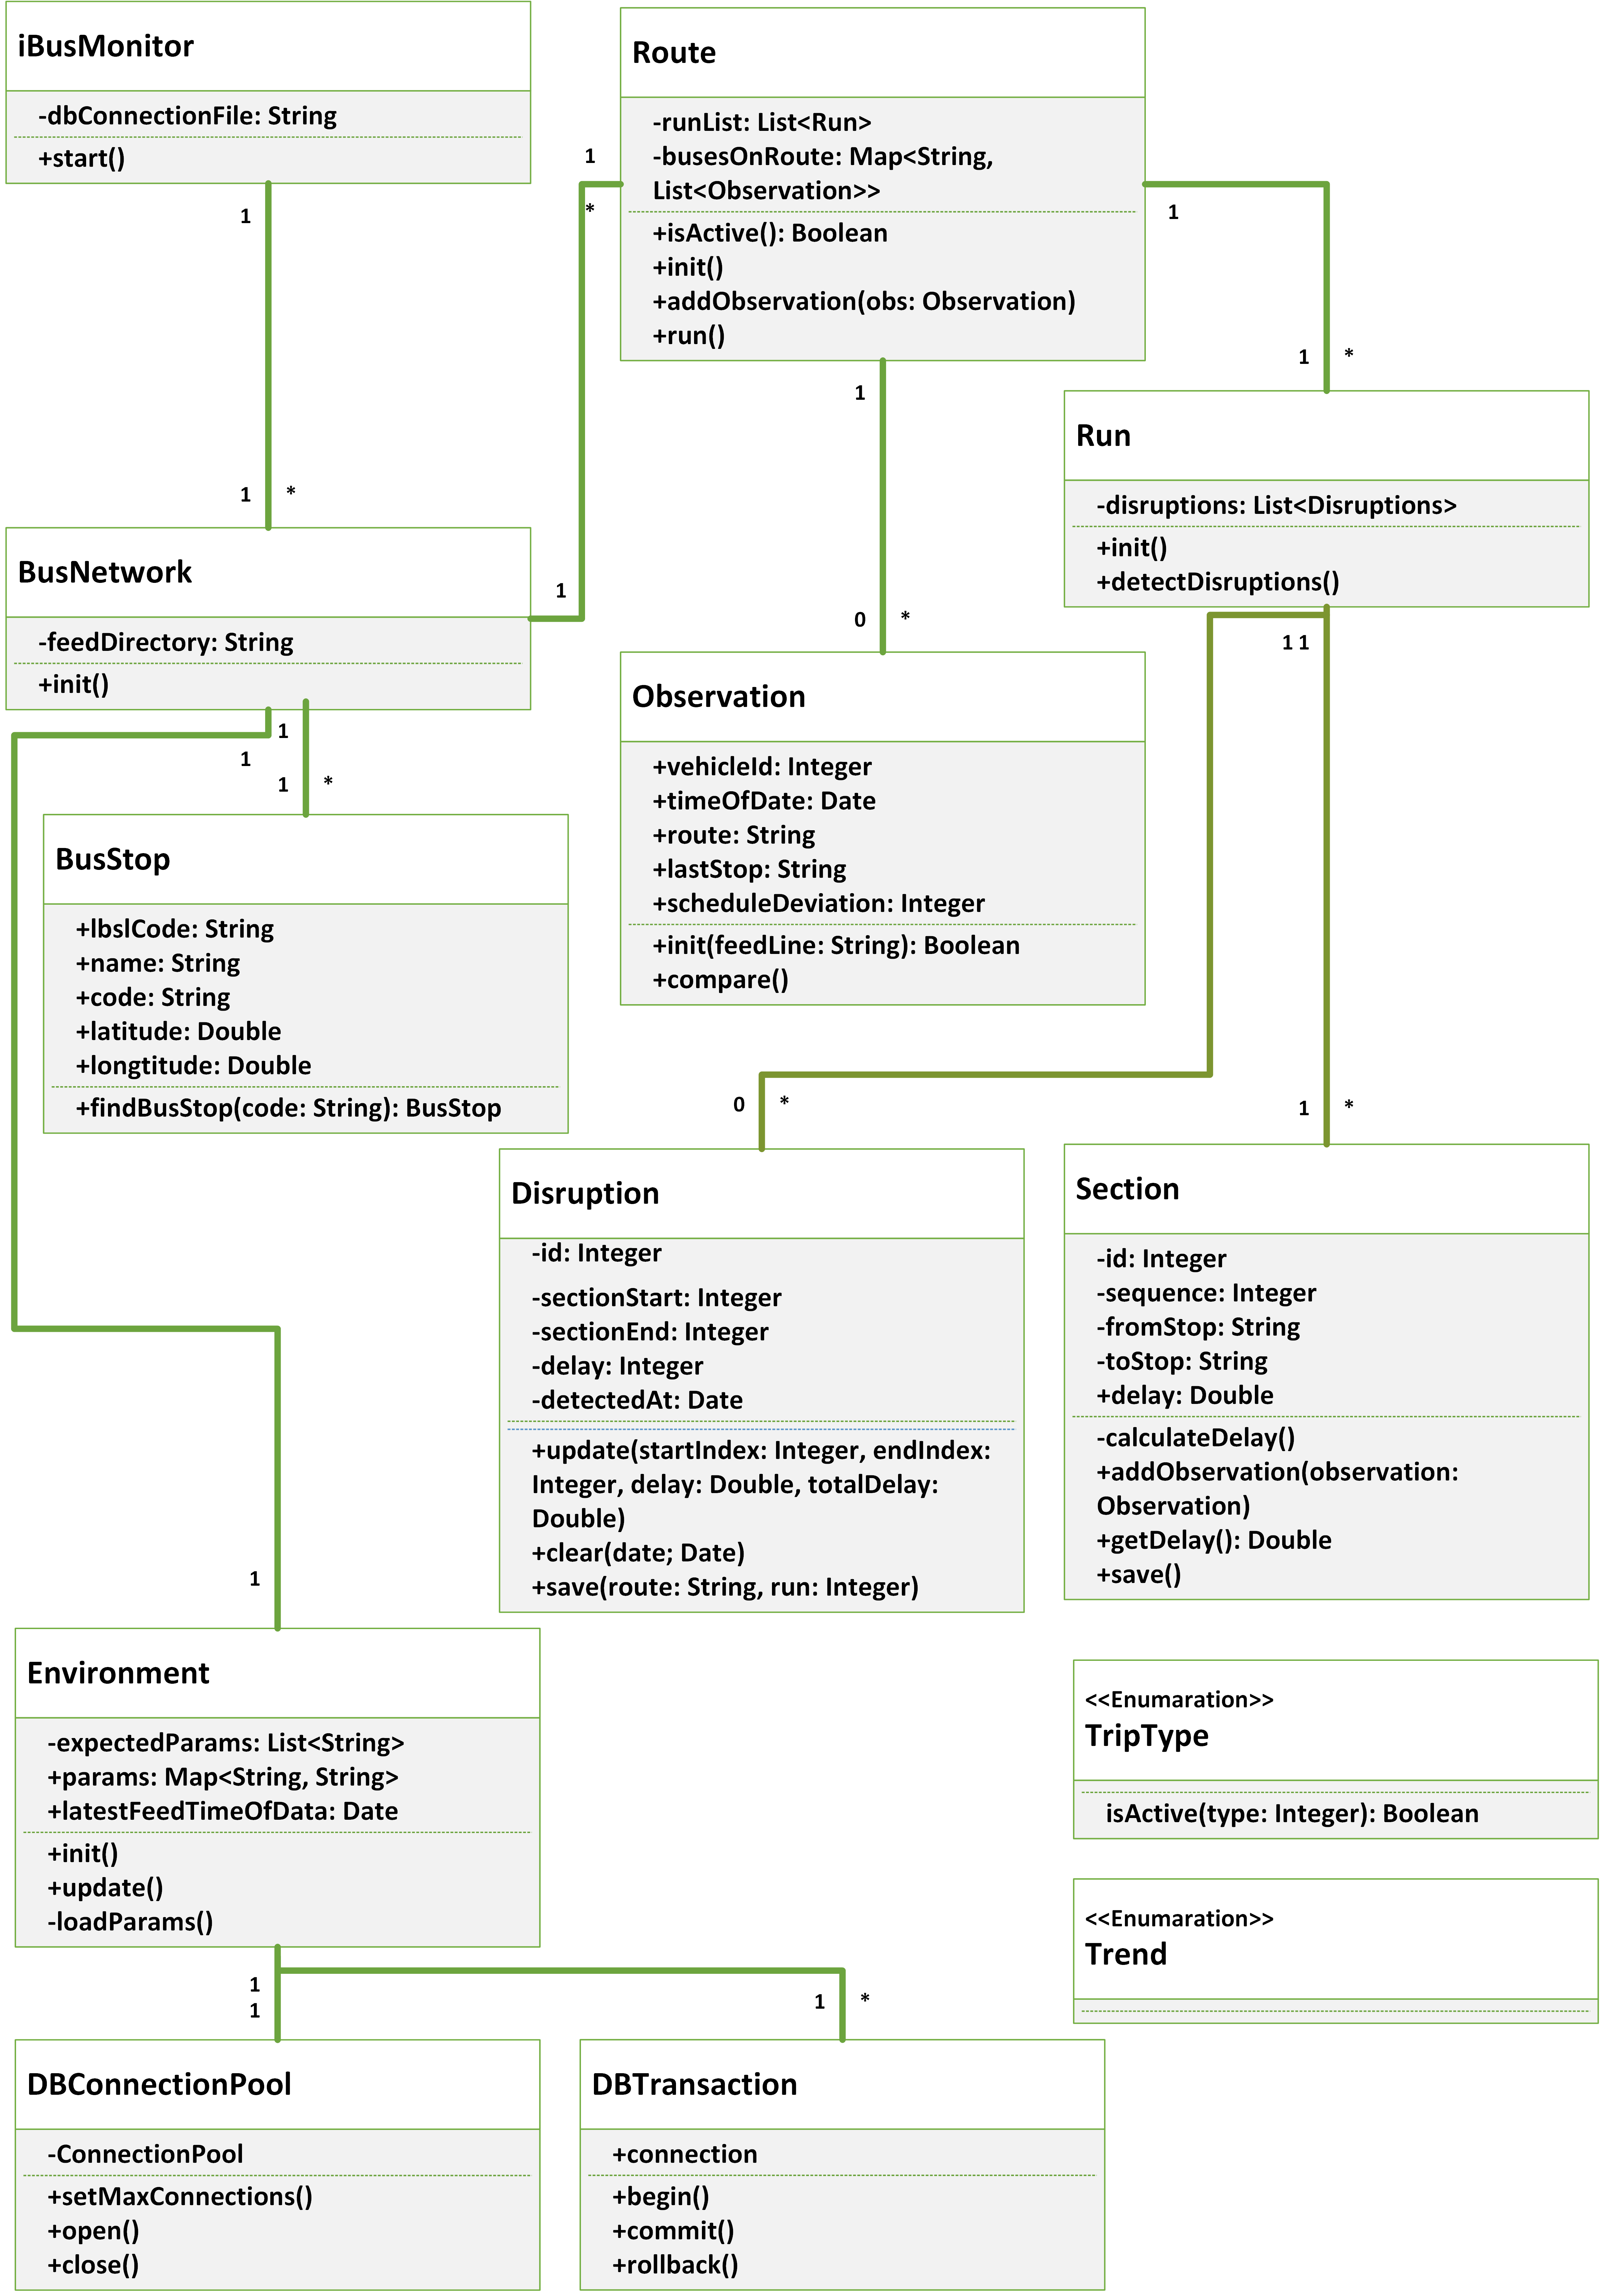
\includegraphics[width=1.2\textwidth]{Figures/Class.png}}
	\caption{Class Diagram}
\label{fig:class}
\end{figure}
%DATABSE MODEL DIAGRAM
\begin{figure}
	\makebox[\textwidth][c]{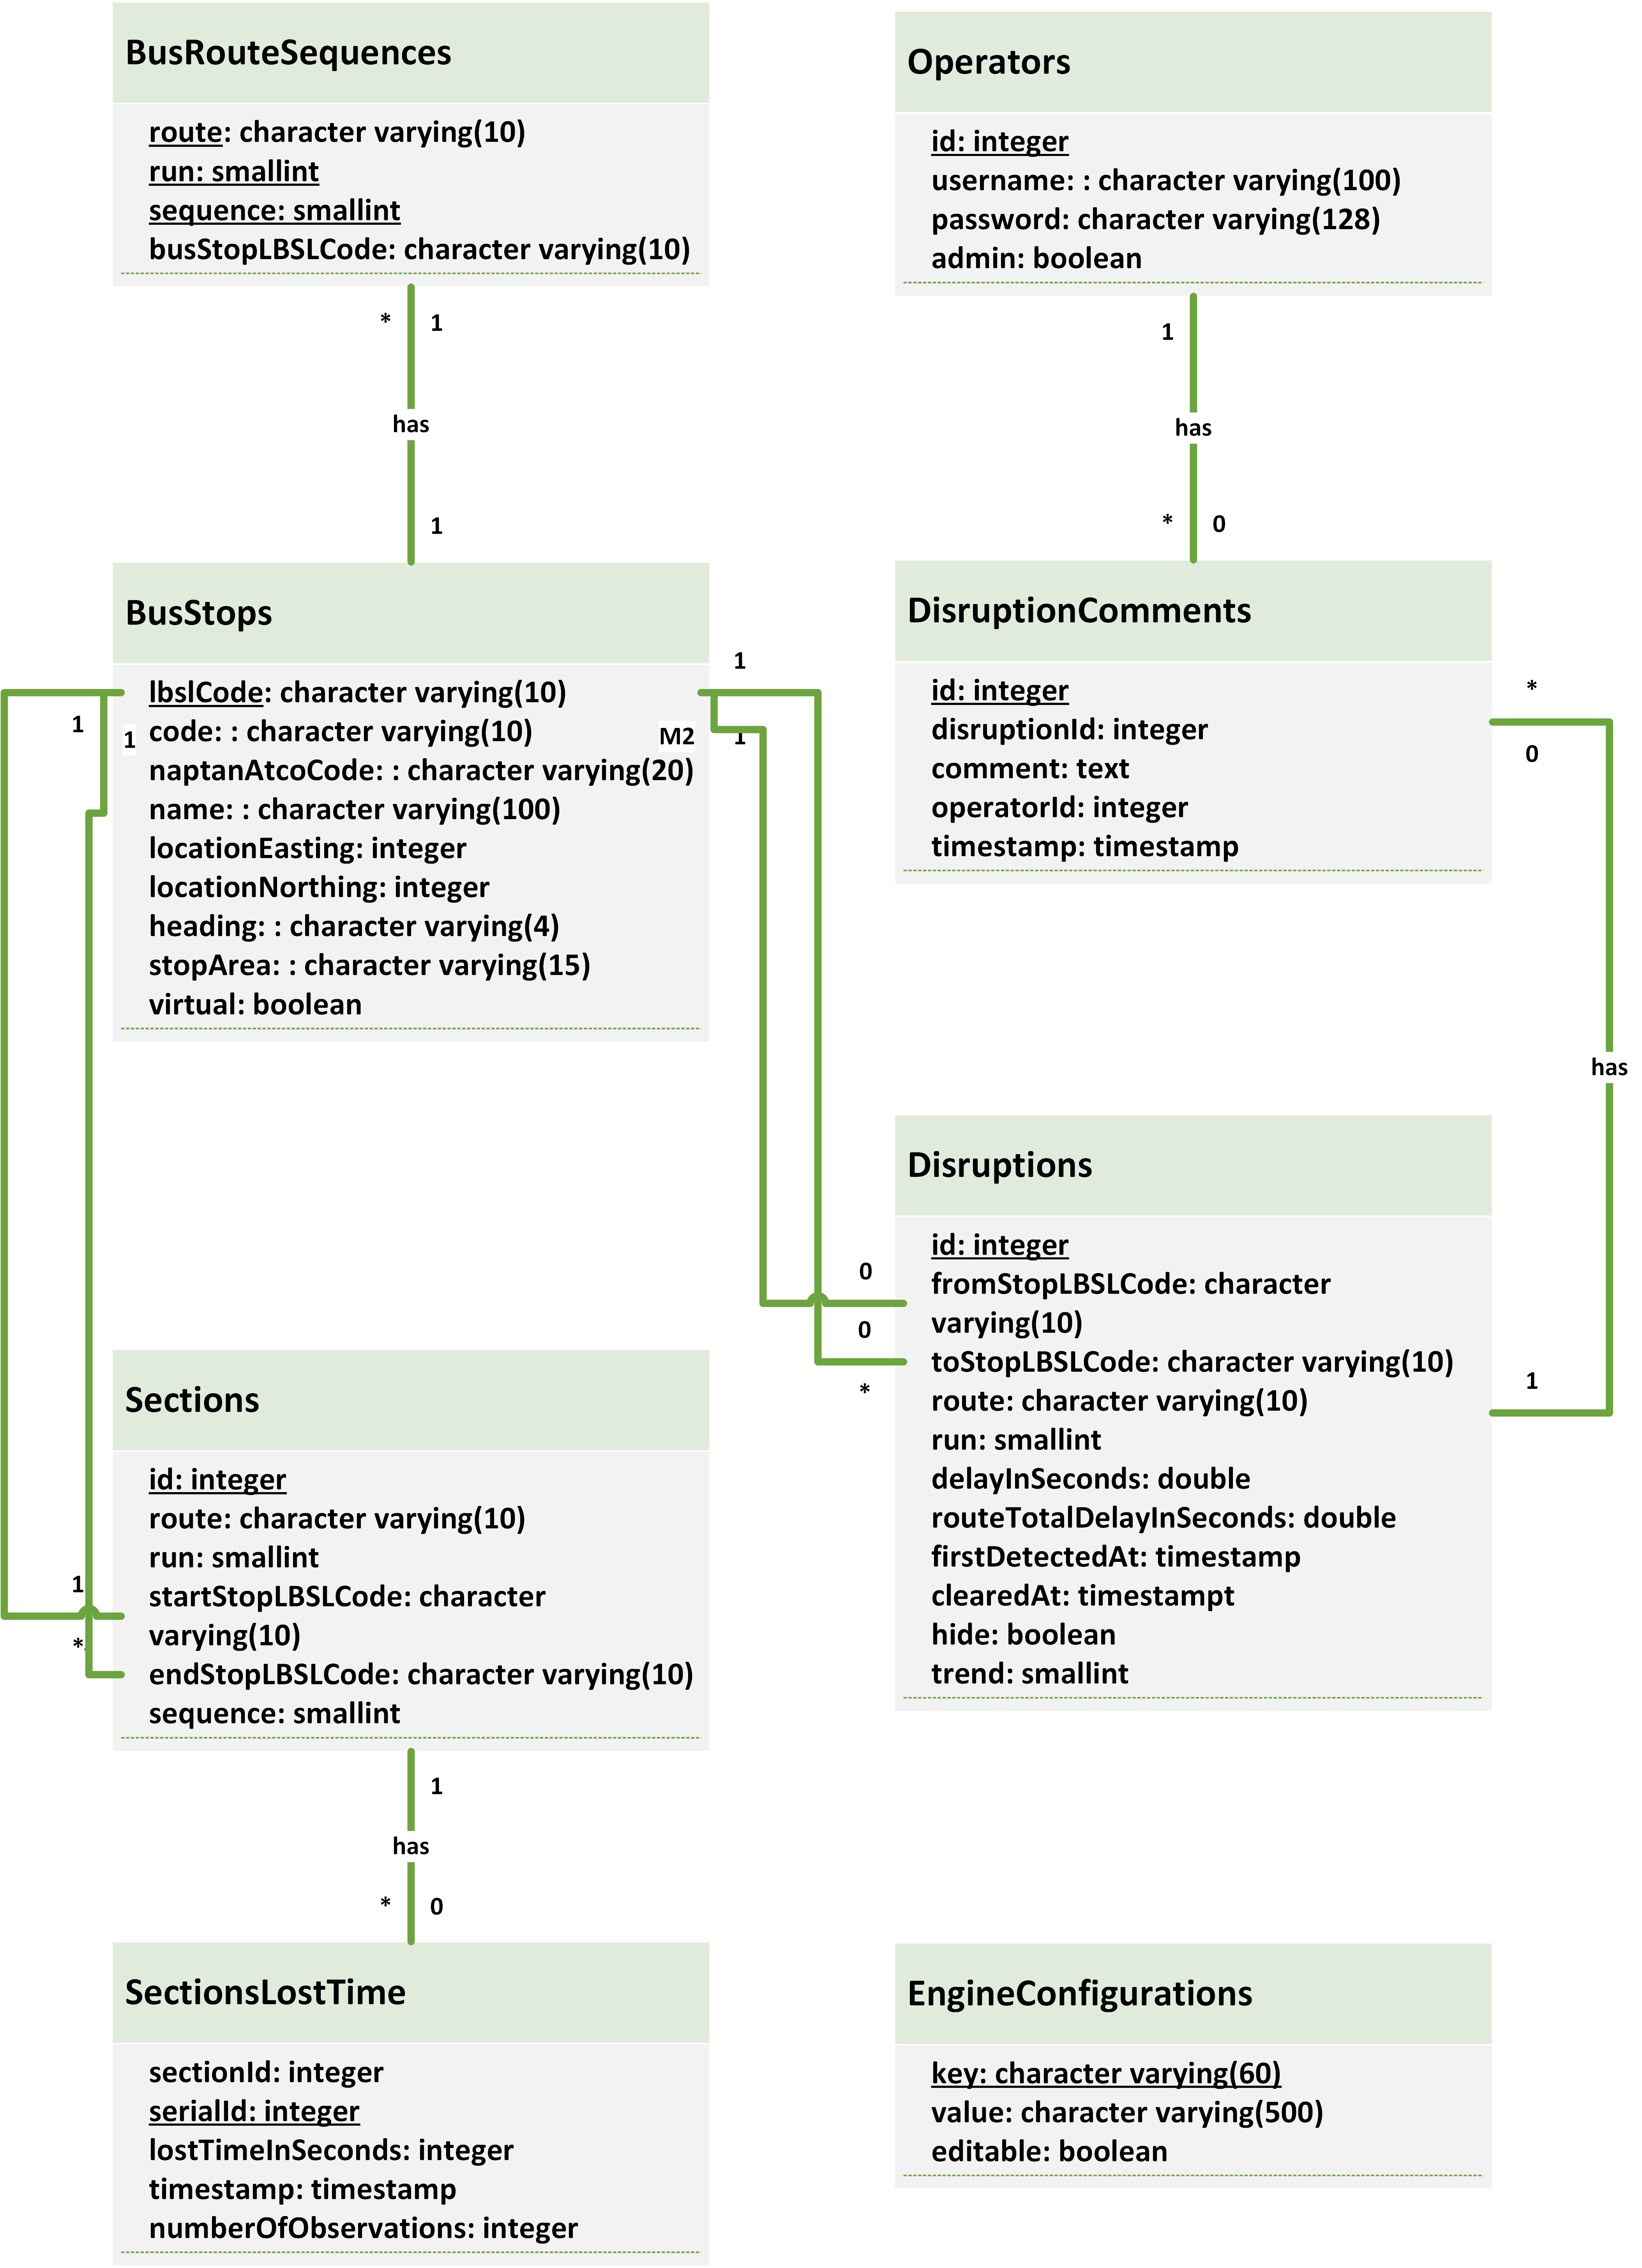
\includegraphics[width=1.2\textwidth]{Figures/DBModel.png}}
	\caption{Database Model Diagram}
\label{fig:dbModel}
\end{figure}
%STATE MACHINE DIAGRAM
\begin{figure}
	\makebox[\textwidth][c]{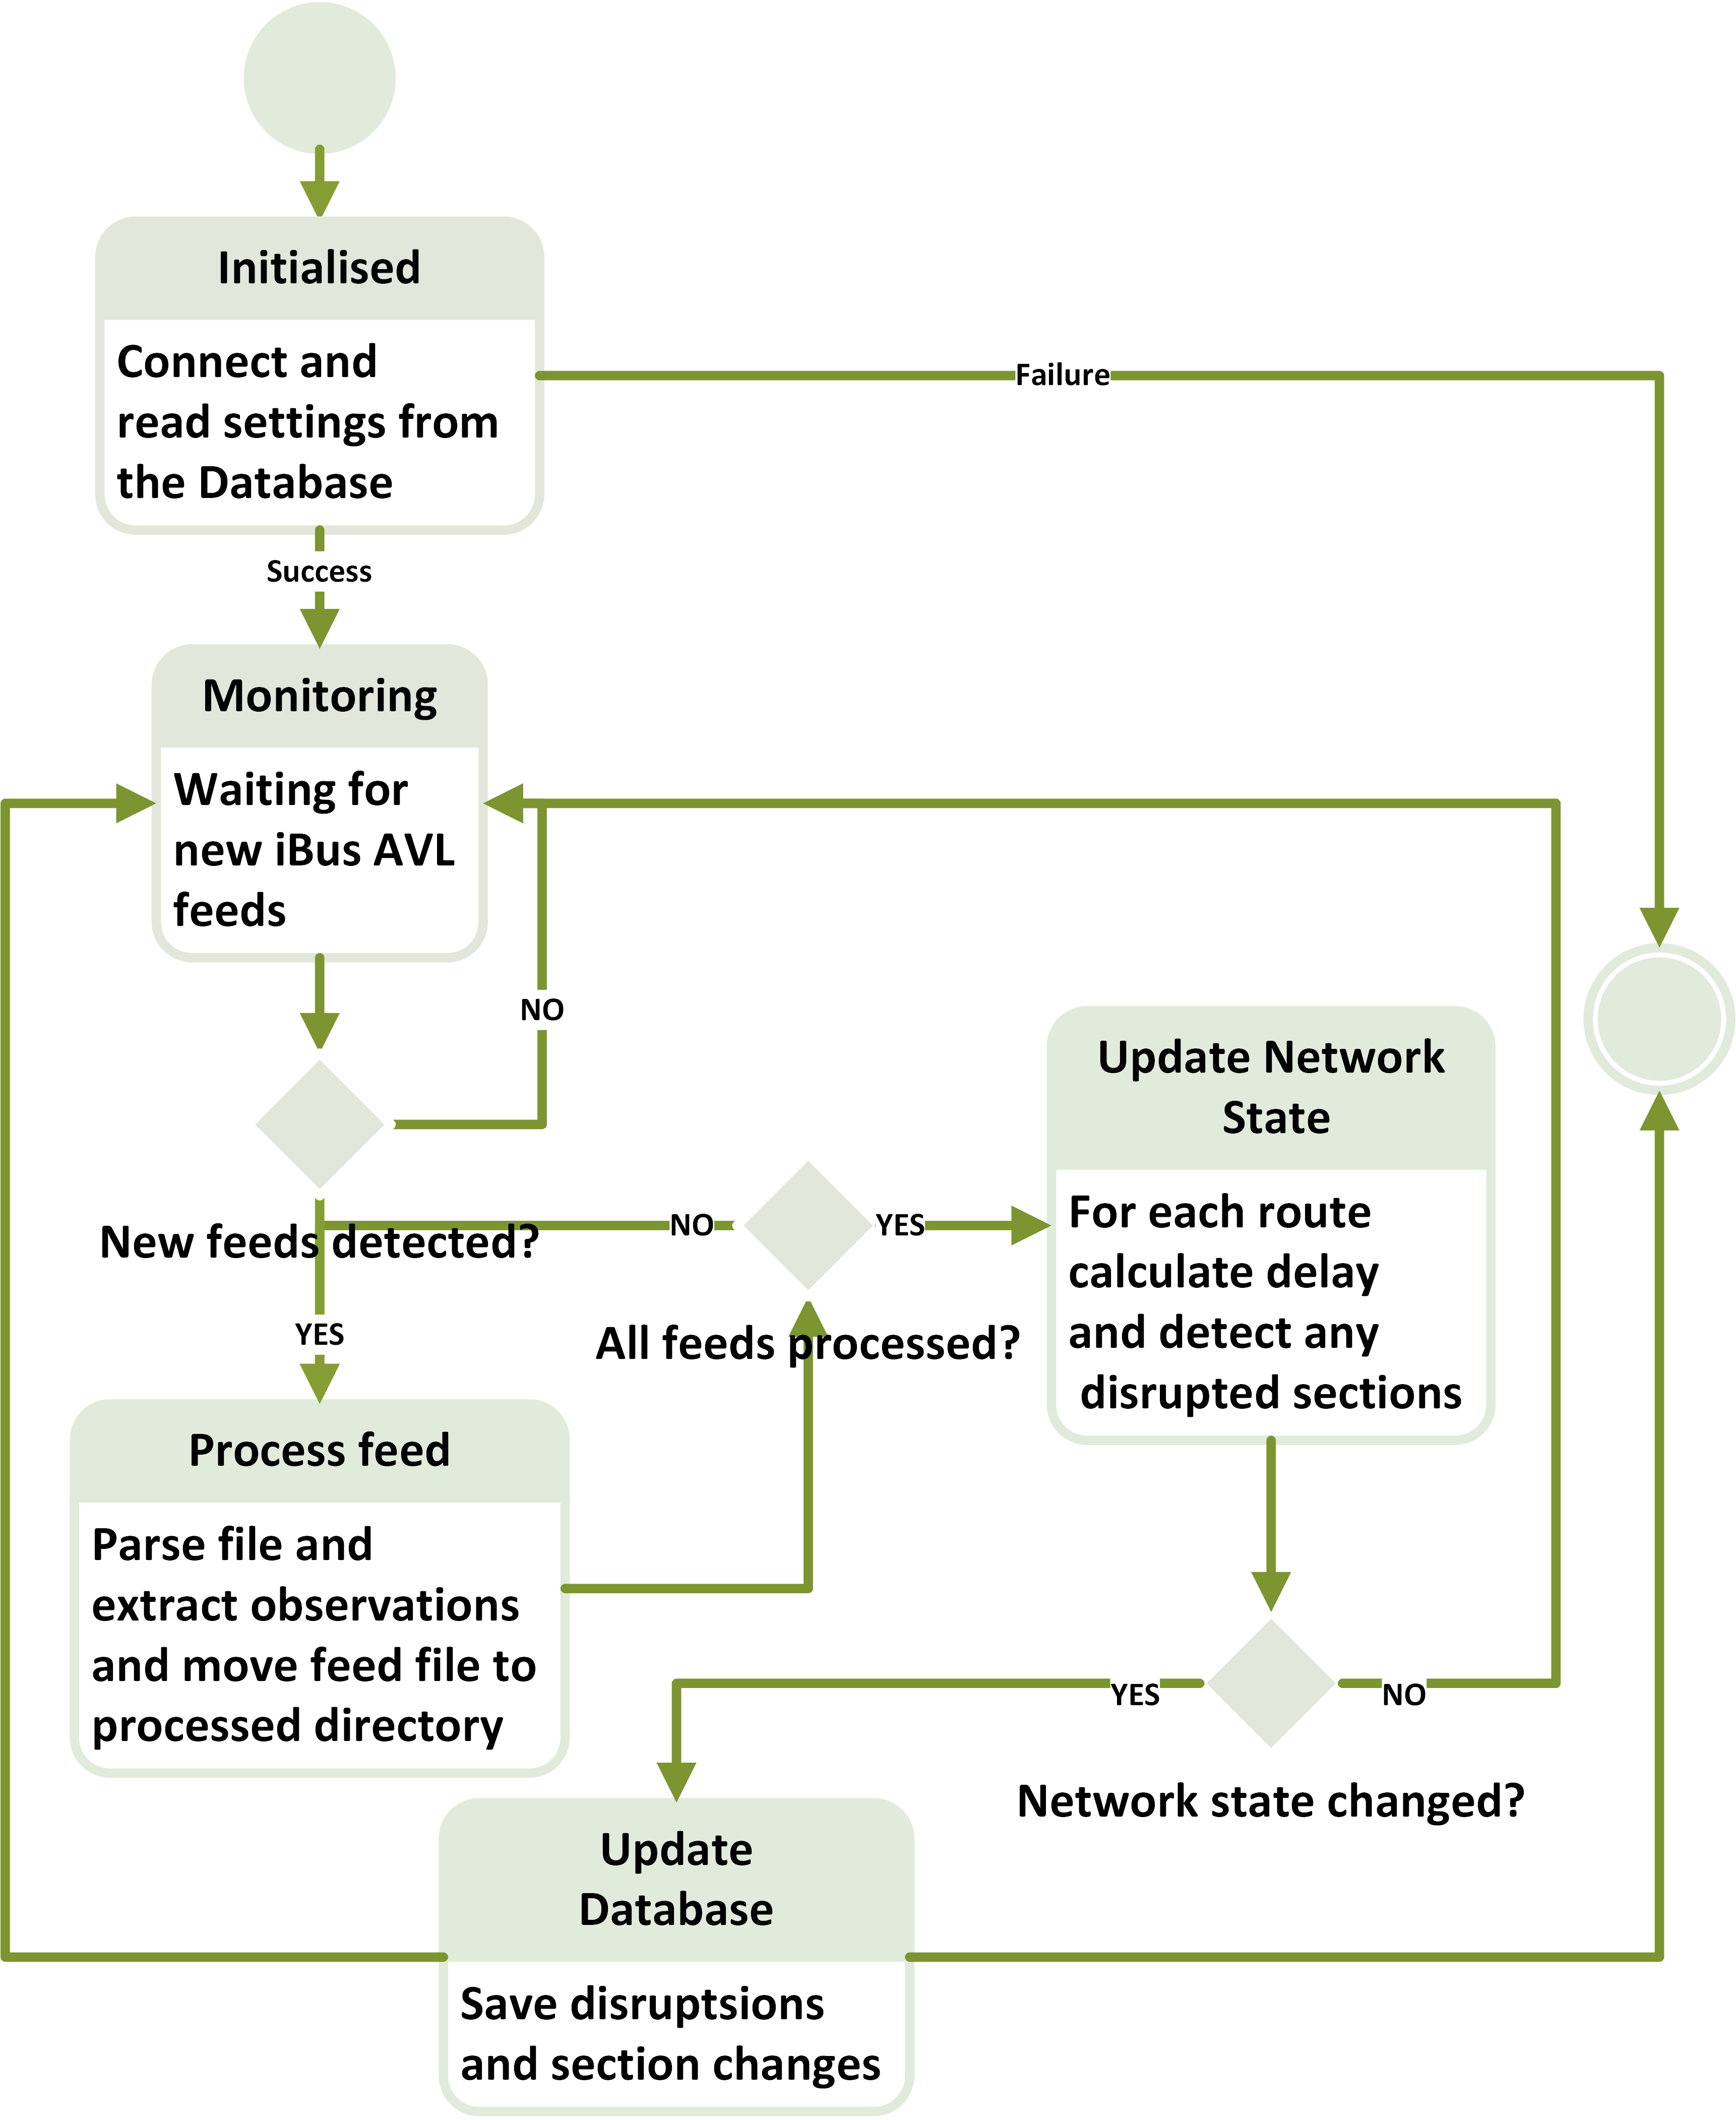
\includegraphics[width=1.2\textwidth]{Figures/StateDiagram.png}}
	\caption{State Machine Diagram}
\label{fig:stateMachine}
\end{figure}

\FloatBarrier
\section{Test Results}

\section{iBus AVL Data Sample}
\begin{figure}[ht!]
	\makebox[\textwidth][c]{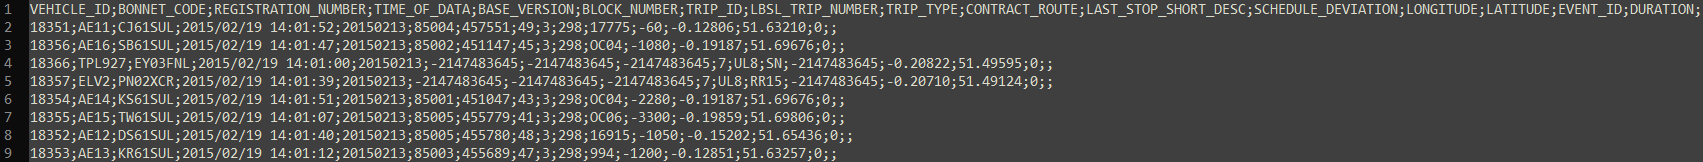
\includegraphics[width=1.7\textwidth]{Figures/ibusSampleRaw.png}}
	\caption{Sample Raw iBus Data}
\label{fig:rawDataSample}
\end{figure}

\begin{figure}[ht!]
	\makebox[\textwidth][c]{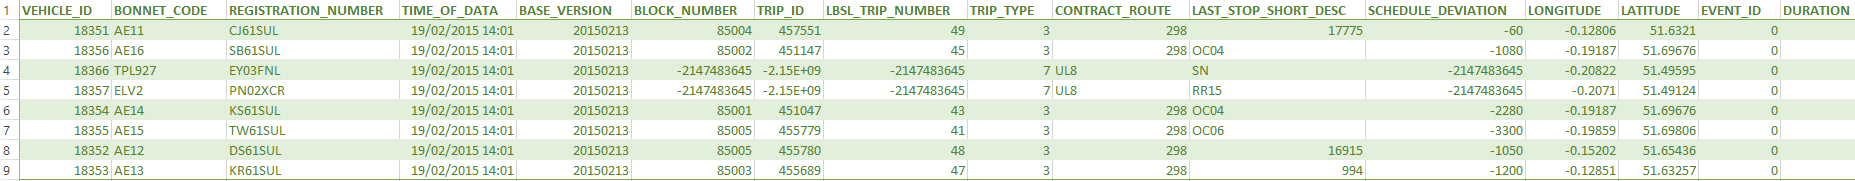
\includegraphics[width=1.7\textwidth]{Figures/ibusSampleFormatted.png}}
	\caption{Formatted Sample iBus Data}
\label{fig:formattedDataSample}
\end{figure}

\FloatBarrier